\chapter{Related Work}
\label{cha:RelatedWork}

\section{Previous Work at ScaDS.AI}

This thesis builds directly upon the foundational work conducted by König \autocite{konig2022model}, Flach \autocite{flach2023methods}, Schaller \autocite{schaller2023train}, and Schneeberger \autocite{schneeberger2024end}, continuing the exploration of autonomous driving agents in the field of machine learning. König's thesis is the earliest work among them. His focus was on training a model to navigate through an obstacle course composed of block-like barriers in a simulated setting. The structure of his obstacle course closely resembles the one used in this work, with a key distinction: the present thesis standardizes the obstacles by making them uniformly red and arranging them in pairs, which requires the vehicle to consistently pass between them, adding a layer of spatial precision to the navigation challenge.

König \autocite{konig2022model} employed a reinforcement learning methodology, specifically leveraging an evolution-based training approach. In contrast to the approach taken in this thesis, König \autocite{konig2022model} utilized an OpenCV-based image processing pipeline to identify obstacles and arena boundaries within the input images. These visual elements were then encoded into tensors that directly represented their spatial properties. As a result, there was no need for a Convolutional Neural Network (CNN), since the network was not required to extract spatial features from raw image data. Instead, a standard Artificial Neural Network (ANN) architecture was sufficient for his setup. His results demonstrated that the model successfully learned to handle a variety of generated obstacle configurations, showing a high degree of generalization across different courses. He concluded that the trained agent was capable of completing most of the parkour-style tracks effectively.

The work of Flach \autocite{flach2023methods} was a direct continuation of König’s earlier research \autocite{konig2022model}, with a focus on addressing one of the most significant challenges in autonomous agent development: bridging the Simulation-to-Reality (Sim2Real) gap. While König concentrated on training the agent within a controlled simulated environment, Flach aimed to transfer the trained model to a real-world setting. This step was crucial for validating whether behaviors learned in simulation could generalize effectively to physical environments. Flach \autocite{flach2023methods} used the same JetBot vehicle and physical arena that are also employed in the current thesis.

However, the transition to the real environment introduced several technical difficulties. One of the primary challenges was the difference in control dynamics between the simulated and physical JetBot vehicles, which made direct transfer of control strategies problematic. Additionally, Flach relied on an OpenCV-based visual processing pipeline, similar to König, which proved to be unreliable under varying real-world lighting conditions. The pipeline often misinterpreted background objects as obstacles and was particularly sensitive to brightness fluctuations, leading to inconsistent performance. The inability of the pipeline to detect object consistently has lead to the refuse to continue the research with the real world experiments and need in usage of the synthesized data. All these problems and differences have lead to the failure of transitioning the model from simulation to reality.

Schaller \autocite{schaller2023train} extended the research done by König \autocite{konig2022model} in addressing the main inaccuracies in his approach and the main problems that occurred during the Flach's \autocite{flach2023methods} research. His work addressed four central research questions, focusing on the feasibility of modeling autonomous driving as an RL problem, effective processing of camera input, overall learning performance, and the robustness of the algorithms under external influences. To achieve this, he developed four RL algorithms using carefully designed state representations and reward functions. These models demonstrated strong performance, particularly on easy and medium tracks, with the PPO-MEM-SGT algorithm even managing to complete the most challenging courses. Instead of using a convolutional neural network, Schaller \autocite{schaller2023train} extracted key coordinates from camera images to construct the state input, showing that simpler preprocessing can yield efficient results.

Schneeberger \autocite{schneeberger2024end} focused on developing a robust autonomous driving agent capable of adapting to varying lighting conditions. His approach employed an end-to-end trained Convolutional Neural Network (CNN), enabling the agent to directly learn control policies from raw visual input without relying on handcrafted feature extraction or preprocessing pipelines. The driving task was structured as a sequence of navigation goals across three difficulty levels, each presenting increasingly complex spatial configurations. The agent was evaluated under three distinct lighting conditions (bright, standard, and dark) designed to test its adaptability and generalization in diverse visual environments.

The results demonstrated that the CNN-based agent performed reliably across all difficulty levels and lighting settings, indicating a high degree of robustness and learning efficiency. By successfully addressing the limitations posed by inconsistent illumination (a challenge that had hindered earlier works) Schneeberger’s \autocite{schneeberger2024end} research marked a significant step forward in the development of more resilient autonomous driving systems.

\section{Imitation Learning}
The foundational paper on Imitation Learning is often credited to Pomerleau \autocite{NIPS1988_812b4ba2}. In this pioneering work, Pomerleau introduced a method for training a self-driving vehicle using a neural network that learns directly from human driving behavior. The approach, known as behavioral cloning, involved collecting image data from a forward-facing camera along with corresponding steering commands from a human driver. A neural network was then trained to map visual input to steering outputs, effectively imitating the demonstrated behavior. This paper laid the groundwork for the field of imitation learning by showing that autonomous control policies could be learned from demonstration rather than being manually programmed, opening the door to a range of data-driven approaches for robotics and autonomous systems.

The paper by Billard et al. \autocite{bakker1996robot} provides a comprehensive survey of imitation learning in the context of robotics, highlighting its potential as a natural and efficient framework for programming autonomous agents. The authors discuss key concepts, such as the distinction between mimicry and emulation, the challenges of mapping observed human actions to robot motor commands, and the importance of generalization beyond direct demonstrations. The paper categorizes imitation learning methods into different approaches, including behavioral cloning, inverse reinforcement learning, and correspondence mapping, offering insights into their strengths and limitations. By bridging insights from neuroscience, cognitive science, and machine learning, this work lays a conceptual foundation for designing robots that learn complex tasks by observing others, and it remains a seminal reference in the field.

\subsection{Imitation Learning Taxonomies}
Imitation Learning (IL) is traditionally categorized into two main approaches: Behavioral Cloning (BC) and Inverse Reinforcement Learning (IRL). Both branches have evolved by integrating diverse techniques and have been adapted to various application domains. Fundamentally, BC and IRL differ in how they aim to replicate expert behavior. BC typically learns a direct mapping from observed states to corresponding actions using supervised learning, whereas IRL focuses on inferring the underlying reward function that would make the expert's actions appear optimal. This fundamental distinction may explain why BC methods are more commonly deployed in real-world applications, while IRL remains largely confined to simulated environments, where the complexity and variability are easier to manage. \autocite{zheng2022imitationlearningprogresstaxonomies}

The definition of Behavioral Cloning (BC) was first proposed in \autocite{bain1995framework}. In this framework, BC is formulated as a supervised learning problem where the goal is to recover an expert policy $\pi_E$ from a set of demonstrations. Assume we observe a trajectory of state-action pairs ${(X_t, A_t)}_{0 \le t \le T}$, where the expert selects actions according to an unknown policy $\pi_E$, i.e., $A_t \sim \pi_E(\cdot \mid X_t)$. To imitate this behavior, we define a parametric policy class ${\pi\theta}_{\theta \in \mathbb{R}^d}$ and seek parameters $\theta$ that minimize a loss function between the learned policy and the expert’s observed behavior. A common approach is to minimize the empirical risk:
\[
  J_T(\pi_\theta) = \sum_{x \in \mathcal{X}} \sum_{a \in \mathcal{A}} \hat{\mu}_T(x) \left( \pi_\theta(a \mid x) - \hat{\pi}_{E,T}(a \mid x) \right)^2,
\]
where $\hat{\mu}_T(x) = \frac{1}{T+1} \sum_{t=0}^T \mathbb{I}_{\{X_t = x\}}$
are the empirical occupation frequencies under the expert’s policy, and $\hat{\pi}_{E,T}(a \mid x) = \frac{\sum_{t=0}^T \mathbb{I}\{X_t = x, A_t = a\}}{\sum_{t=0}^T \mathbb{I}\{X_t = x\}}$ is the estimate of expert policy. \autocite{neu2012apprenticeshiplearningusinginverse}

A formal definition of Inverse Reinforcement Learning was first introduced by Russell \autocite{russell1998learning}. In this formulation, the objective is to infer the underlying reward function that an expert is implicitly optimizing, based solely on observations of their behavior. Unlike standard reinforcement learning, where the reward function is known and the goal is to learn a policy, IRL reverses this process by assuming access to expert trajectories and attempting to deduce the reward structure that would make such behavior optimal. This approach is particularly useful in scenarios where specifying a reward function manually is difficult or unintuitive, such as in complex human tasks. Russell’s work laid the theoretical groundwork for a wide range of subsequent research, leading to more advanced IRL algorithms that are now used in robotics, autonomous systems, and human behavior modeling.

Imitation Learning (IL) can also be classified into model-based and model-free approaches, depending on whether the algorithm utilizes a forward model to understand environmental dynamics. In model-based methods, the agent attempts to learn or leverage a model of how the environment responds to actions, while model-free methods bypass this by learning policies directly from data. Historically, most IRL (Inverse Reinforcement Learning) methods have been model-based, as they often require iterative evaluations within the environment to infer the underlying reward function. In contrast, Behavioral Cloning (BC) methods are typically model-free, since they rely on supervised learning and often assume access to a low-level controller. The introduction of Generative Adversarial Imitation Learning (GAIL) \autocite{ho2016generative} marked a shift, enabling IRL-style imitation in a model-free setting. This led to the development of various adversarially structured IL algorithms that follow GAIL’s paradigm.

While incorporating a model of the environment can provide richer contextual information and improve data efficiency, it is not always necessary—or even feasible—depending on the task. Model learning can be both computationally expensive and technically challenging. In domains like robotics, where precise measurements such as position and velocity are easily accessible, the benefits of modeling system dynamics may be minimal. However, in complex scenarios such as autonomous driving, understanding dynamics can be essential for safety, such as avoiding collisions with pedestrians. Ultimately, the choice between model-based and model-free approaches should be guided by the specific demands and constraints of the application. \autocite{zheng2022imitationlearningprogresstaxonomies}

\section{Imitation Learning in Autonomous Driving}

As mentioned earlier, Imitation Learning in autonomous driving traces its roots back to the late 1980s with pioneering projects like Autonomous Land Vehicle In a Neural Network (ALVINN) \autocite{NIPS1988_812b4ba2}. ALVINN was one of the first systems to apply neural networks to autonomous navigation by training a vehicle to mimic human driving behavior. It used a single-layer neural network to map input from a forward-facing camera and a laser rangefinder directly to steering commands. The model was trained using supervised learning from human driving demonstrations, making it an early form of Behavioral Cloning. Despite the limited computational resources of the time, ALVINN successfully drove a van on public roads for extended distances, showcasing the feasibility of learning-based control systems.

\begin{figure}[htbp]
  \centering
  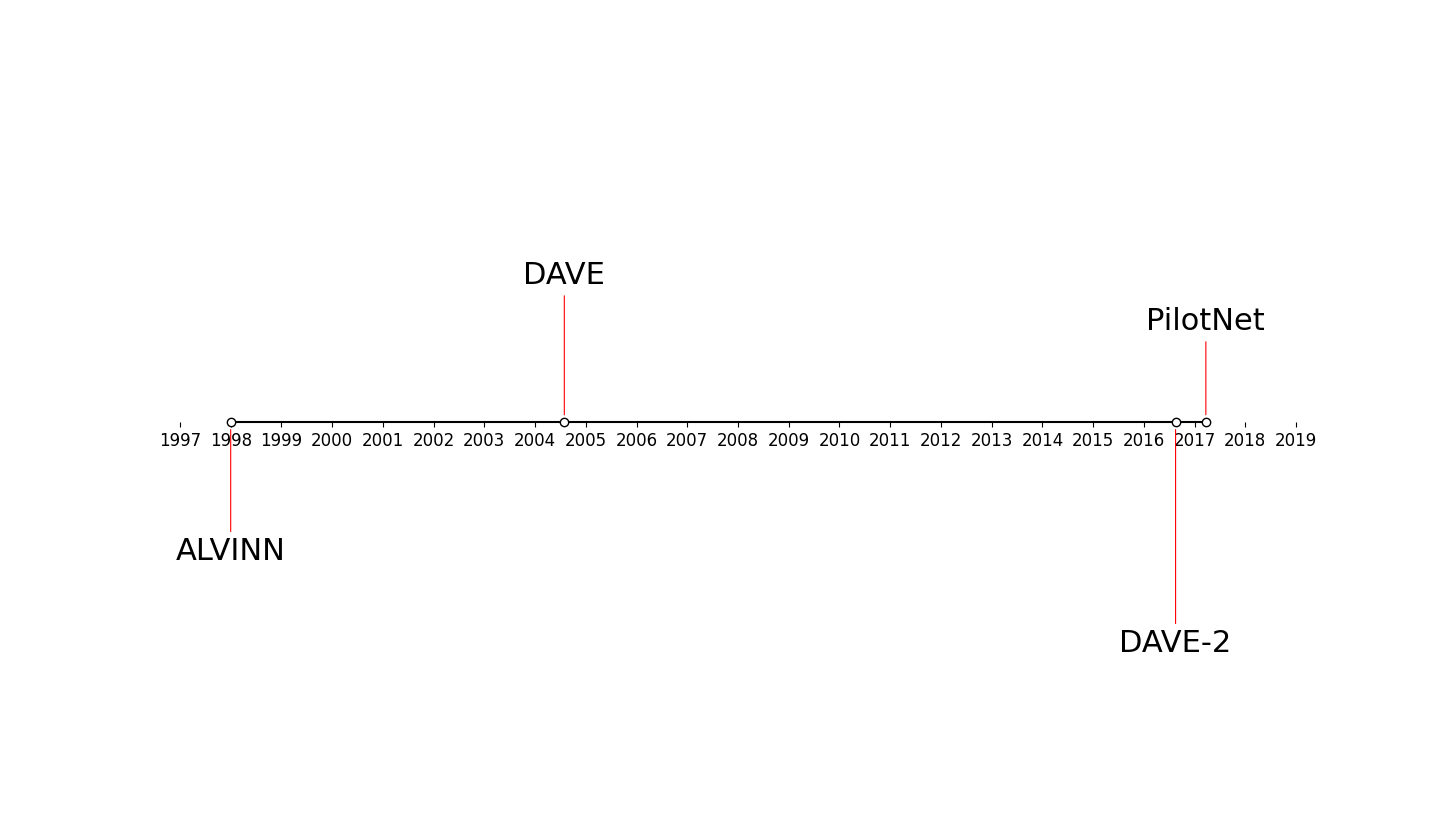
\includegraphics[width=0.9\textwidth]{Images/imitation_learning_timeline.png}
  \caption{Timeline diagram of the most impactful researches in the field of Imitation Learning for Autonomous Driving.}
  \label{fig:imitation_learning_timeline}
\end{figure}

One of the biggest works in application of Behavioral Cloning to autonomous driving was the DAVE project \autocite{muller2004autonomous}, developed in the Defense Advanced Research Projects Agency (DARPA). This early system demonstrated that it was possible to train a neural network to control a vehicle by learning from a dataset that contains only data collected by the camera. They used 2 cameras to collect the images from different perspectives, so that despite not having any other sensors installed on the vehicle, the model would have been able to learn to estimate the depth. As a result they've captured a slightly better performance from the model trained and executed using a binocular setup, rather than the monocular one.

Building on the foundations of DAVE, NVIDIA introduced its own successor, DAVE-2 \autocite{bojarski2016endendlearningselfdriving}, which represented a significant leap forward in autonomous driving research. DAVE-2 utilized a deep Convolutional Neural Network trained entirely using Behavioral Cloning. By processing raw pixel data from front-facing cameras, the network could learn to output steering angles, demonstrating impressive lane-following capabilities in real-world environments. The CNN architecture of many other works about autonomous driving was inspired by DAVE-2. List of such works includes the paper from Farag et al. \autocite{8855753}, on which this thesis was mostly based on and whose architecture was used (with certain adjustments) for the CNN architecture in this work. The idea of using the LSTM layers \autocite{6795963} was also inspired by the "Future work" section of this paper.

In addition to DAVE-2, NVIDIA also developed PilotNet, which became their first autonomous driving system capable of navigating highways with minimal human intervention. They've utilized a much more sophisticated CNN architecture, which includes residual \autocite{he2015deepresiduallearningimage}, convolutional and fully connected layers. In contradiction to previous autonomous systems, PilotNet's output is not just a steering angle, but rather a driving trajectory. The reasoning behind using this approach is that the steering angle doesn't fully represent the decision-making process of the car driver, which in it's turn is dictated by the car's geometry, slope and obstacles on the road. PilotNet was designed to produce the three-dimensional trajectory, that would then be fed into an independent controller guiding the car along it. Like its predecessors, PilotNet followed an end-to-end learning paradigm, relying on supervised learning from human drivers. This system marked a practical transition from research prototypes to road-capable AI systems, showcasing the effectiveness of Behavioral Cloning for structured environments such as highways.
